\bfseries

\title[\textsc{Madagascar} Software Package]{Reproducible Computational Experiments  Using \\ \textsc{Madagascar} Software Package}

\author[S. Fomel] % (optional, nur bei vielen Autoren)
{Sergey~Fomel}
% - Der \inst{?} Befehl sollte nur verwendet werden, wenn die Autoren
%   unterschiedlichen Instituten angeh�ren.

\institute[2nd Annual Scientific Software Days] % (optional, aber oft n�tig)
{
  Bureau of Economic Geology \\
  Jackson School of Geosciences \\
  The University of Texas at Austin
}

\date{May 15, 2008}

\setbeamercolor{quotecol}{fg=black,bg=white}

\newcommand{\quotebox}[3]{
  \begin{beamercolorbox}[wd=\textwidth,center]{quotecol}
    \begin{quote}
      #1 
      \color{blue}{\emph{#2}, #3}
    \end{quote}
    \end{beamercolorbox}
}

\begin{frame}
  \titlepage
\end{frame}

\section{The Magic of Science}

\begin{frame}
  \MadLogo
  \frametitle{Outline}
  \tableofcontents[pausesections]
\end{frame}

\begin{frame}<beamer>
  \MadLogo
  \frametitle{Outline}
  \tableofcontents[currentsection]
\end{frame}

\begin{frame}
\MadLogo
\frametitle{The Magic of Science}

\begin{center}
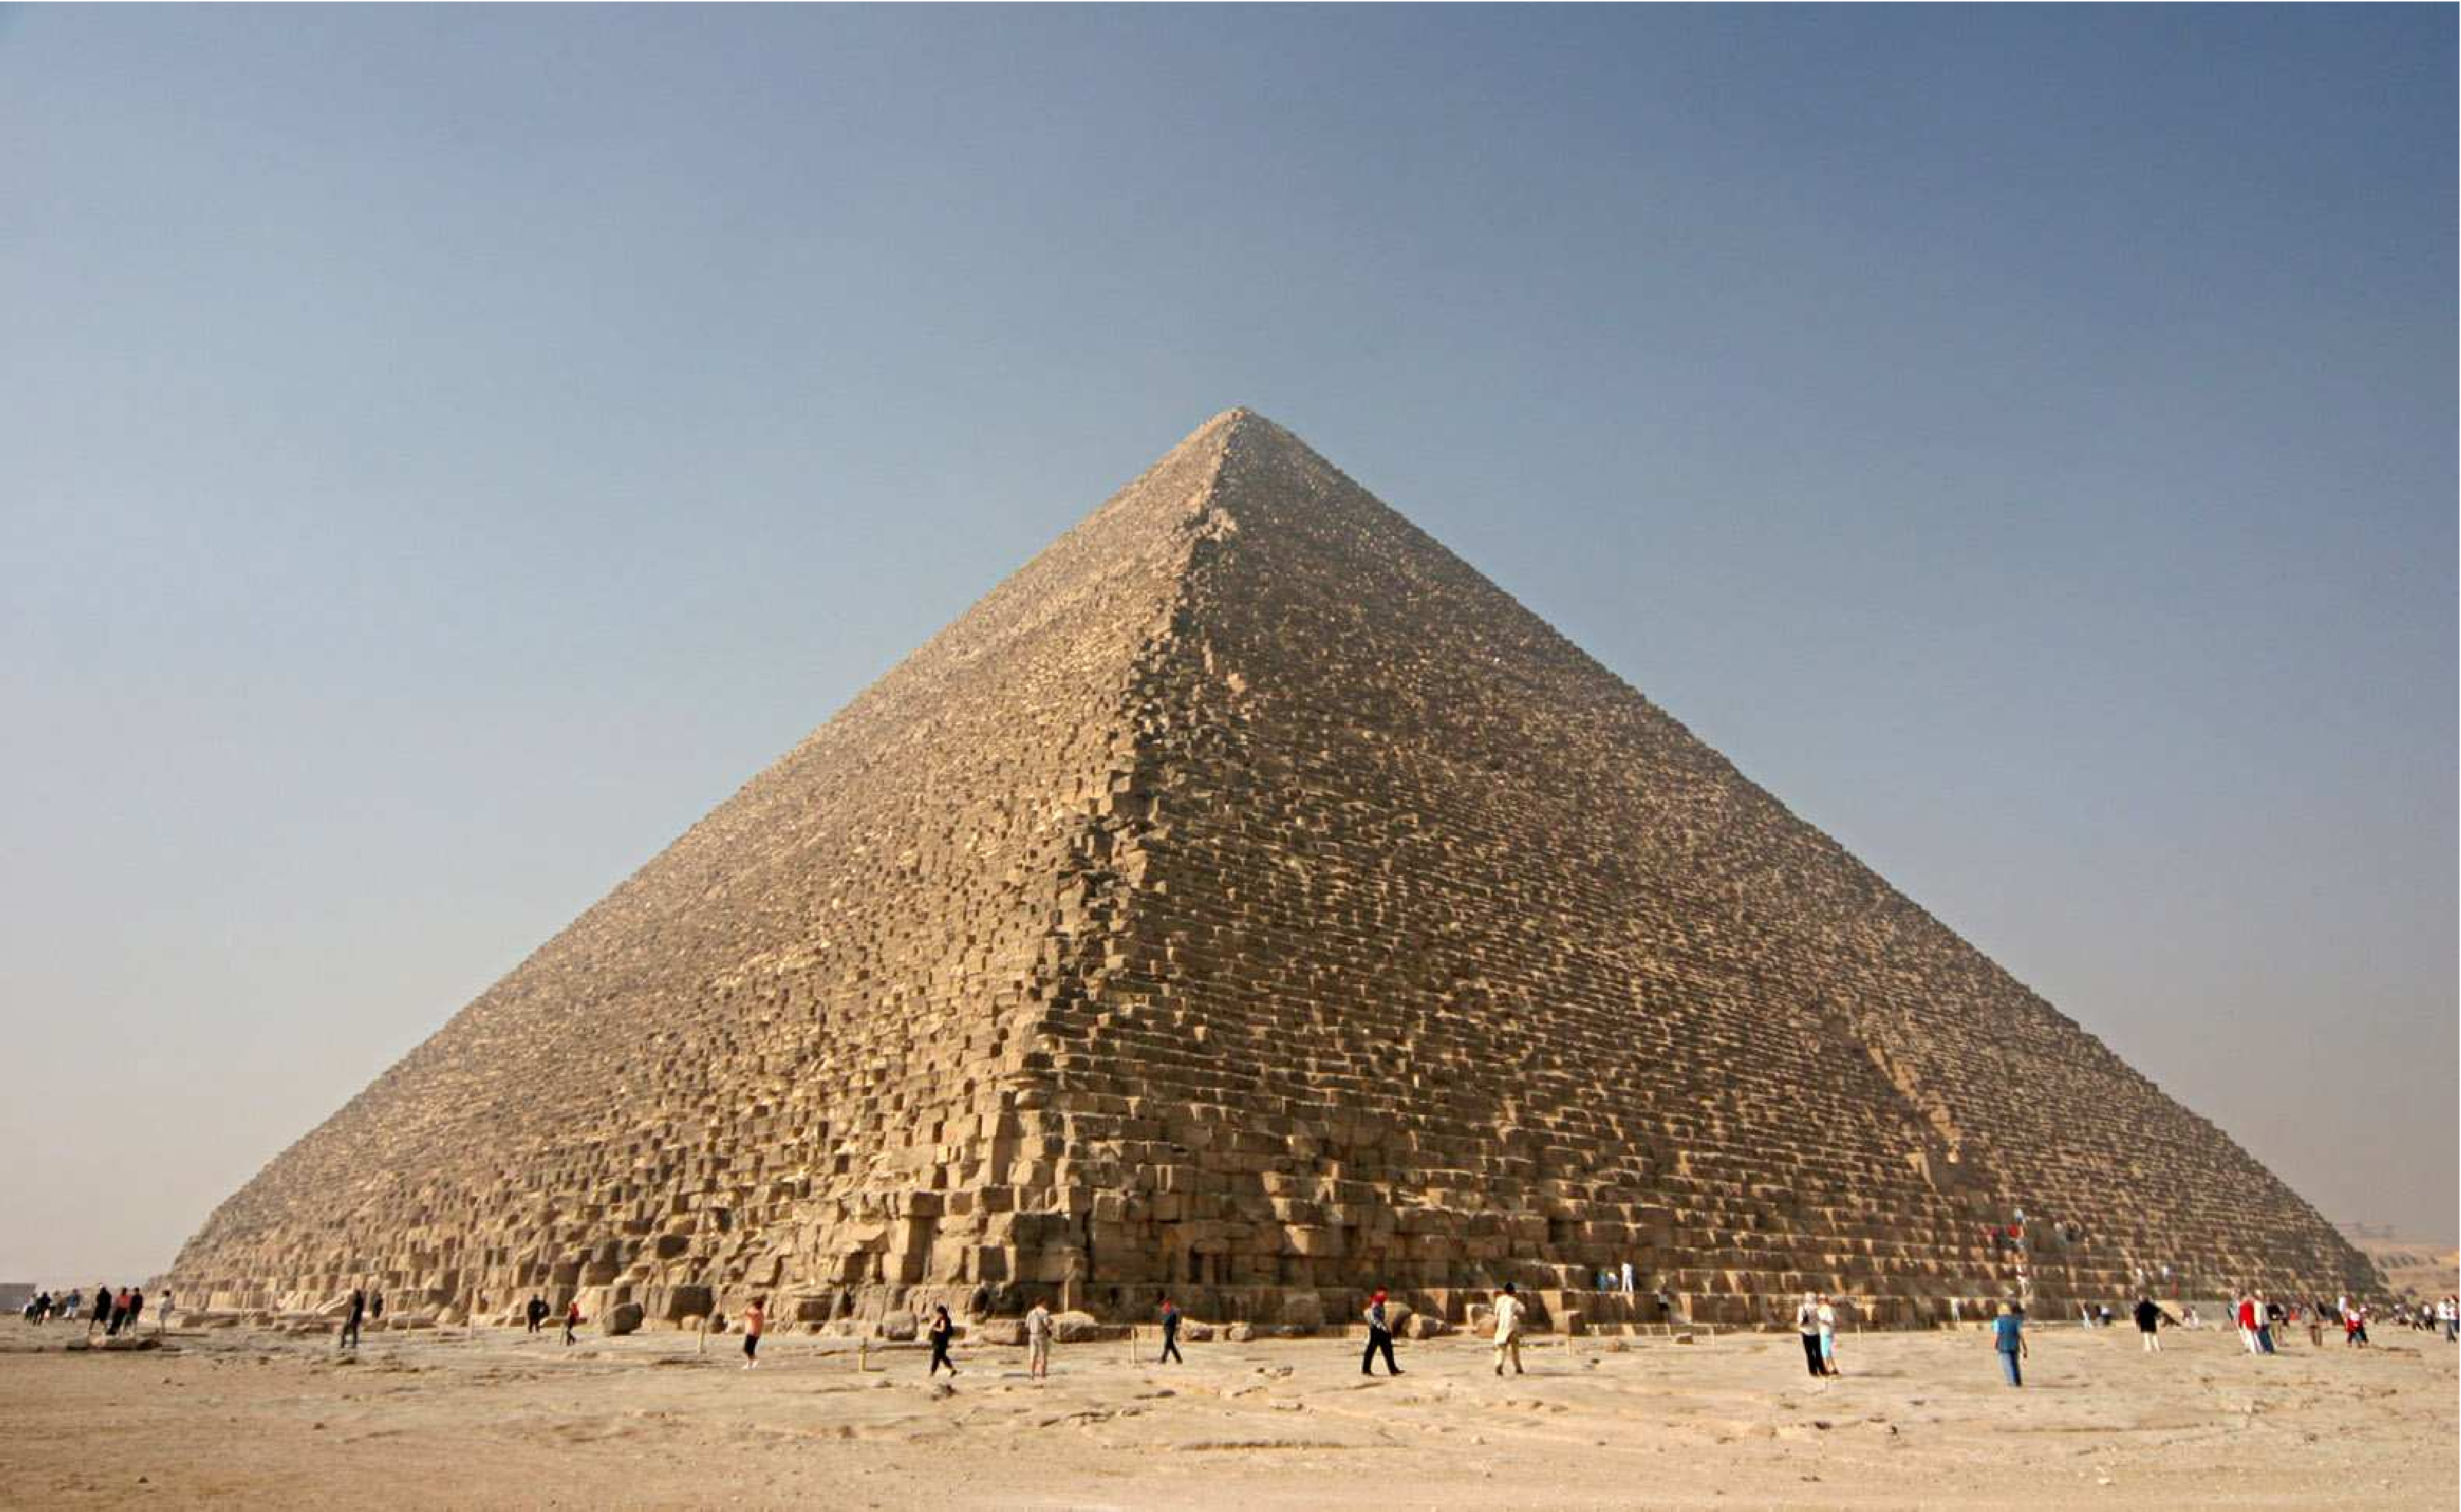
\includegraphics[height=0.6\textheight]{Fig/Kheops-Pyramid}

\begin{itemize}
\item Verification and Validation
\item Reproducibility
\item Peer Review
\end{itemize}

\end{center}

\end{frame}

\begin{frame}
\MadLogo
\frametitle{The Magic of Computer Science}

\begin{itemize}
\item 
\includegraphics[height=0.15\textheight]{Fig/Google}
\end{itemize}

\begin{itemize}
\item \includegraphics[height=0.15\textheight]{Fig/Gnu}

\includegraphics[height=0.15\textheight]{Fig/Tux}
\end{itemize}

\quotebox{Abandoning the habit of secrecy in favor of process
  transparency and peer review was the crucial step by which alchemy
  became chemistry.  In the same way, it is beginning to appear that
  open-source development may signal the long-awaited maturation of
  software development as a discipline.}
{Eric S. Raymond}{TAUP, 2004}

\end{frame}

\begin{frame}
\MadLogo
\frametitle{The Magic of Computational Science}

\quotebox{ 
Within the world of science, computation is now rightly seen as a
third vertex of a triangle complementing experiment and
theory. However, as it is now often practiced, one can make a good
case that computing is the last refuge of the scientific scoundrel [...] 
Where else in science can one get away with publishing observations
that are claimed to prove a theory or illustrate the success of a
technique without having to give a careful description of the methods
used, in sufficient detail that others can attempt to repeat the
experiment? 
}{Randall J. LeVeque}{ICM, 2006}

\end{frame}

\begin{frame}
\MadLogo
\frametitle{(Hale, 1984)}
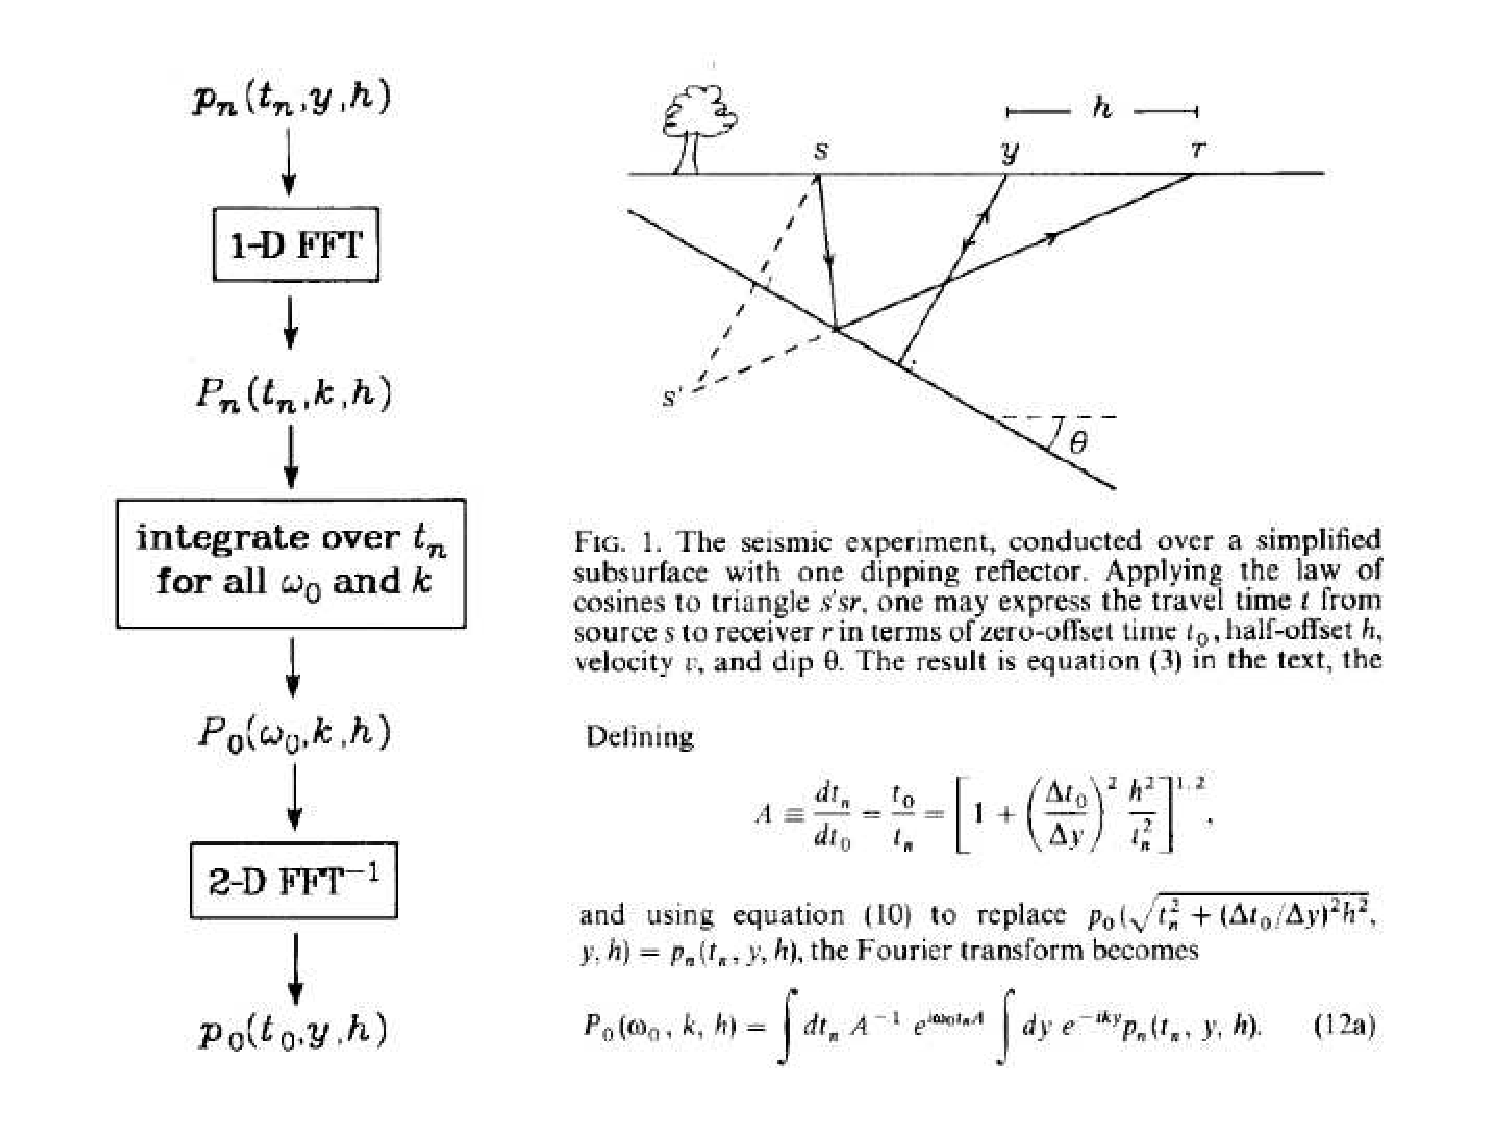
\includegraphics[height=0.8\textheight]{Fig/Hale1}
\end{frame}

\begin{frame}
\MadLogo
\frametitle{(Hale, 1984)}
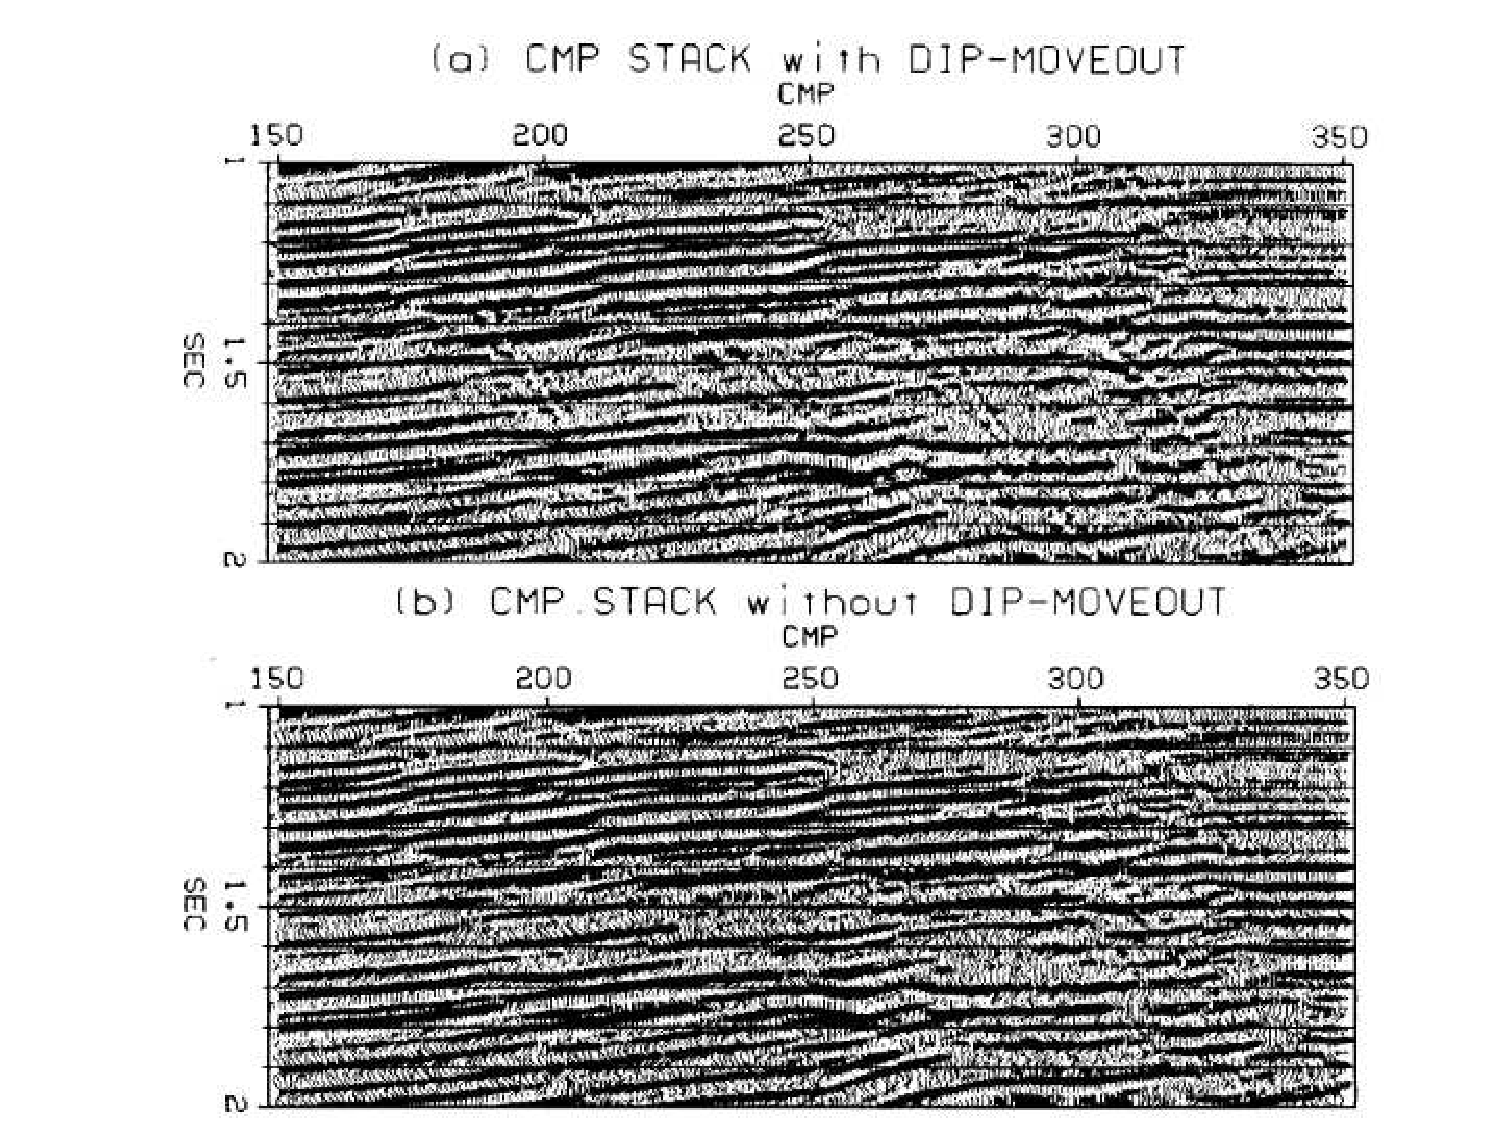
\includegraphics[height=0.8\textheight]{Fig/Hale2}
\end{frame}

\begin{frame}
\MadLogo
  \frametitle{The Magic of Computational Science}
  \quotebox{
An article about computational science in a scientific publication is not the
scholarship itself, it is merely advertising of the scholarship. The actual scholarship
is the complete software development environment and the complete
set of instructions which generated the figures.}
{\\ Jon B. Buckheit and David L. Donoho}{WaveLab, 1995}
\end{frame}

\section{History of Reproducible Research}

\begin{frame}<beamer>
  \MadLogo
  \frametitle{Outline}
  \tableofcontents[currentsection]
\end{frame}

\begin{frame}
  \MadLogo
  \frametitle{Stanford Exploration Project}

  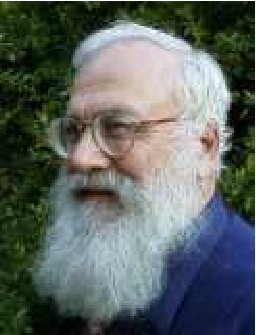
\includegraphics[height=0.2\textheight]{Fig/Claerbout}

  \begin{itemize}
  \item 1 proposal, 60 PhDs 
  \item Electronic books
  \item (Schwab, Karrenbach, and Claerbout, 2000)
  \end{itemize}

\quotebox{
    The purpose of reproducible research is to facilitate someone going a step
    further by changing something. The first step that 
    someone will want to make
    is to be sure that your work is reproducible before they change and improve
    upon it.}{Jon F. Claerbout}{1991}

\end{frame}

\begin{frame}
  \MadLogo
  \frametitle{Follow Up}
  \begin{itemize}
    \item Computational Harmonic Analysis (Donoho et al)
    \item Computational Wave Propagation (LeVeque)
    \item Computational Biostatistics (Gentlemen et al)
    \item Summarized in \emph{CiSE}, Jan/Feb 2009
  \end{itemize}
\end{frame}

\begin{frame}
  \MadLogo
  \frametitle{Lessons}

  \begin{itemize}
  \item {\color{blue}{\Large Reproducibility = Maintenance}}
  \item Community is important
  \item Tools are important
      \begin{enumerate}
      \item Number crunching
      \item Visualization and experiment setup 
      \item Publications and presentations
      \end{enumerate}
  \item Computational experiments are {\color{blue}{tests}}
  \end{itemize}

\end{frame}

\begin{frame}
  \MadLogo
  \frametitle{\textsc{Madagascar} Package}

  \begin{itemize}
    \item Publicly available since 2006
    \item Version 0.9.6
    \item Open source, open community, open science
    \item Vladimir Bashkardin, Jules Browaeys, Cody Brown, Will Burnett, Maria Cameron, Sergey Fomel, Gilles Hennenfent, Trevor Irons, Jim Jennings, Long Jin, 
Yang Liu, Doug McCowan, Henryk Modzelewski, Colin Russell, Paul Sava, Jeffrey Shragge, Eduardo Filpo Silva, Ioan Vlad, Jia Yan
    \item \color{blue}{{\Large \url{http://rsf.sourceforge.net}}}
  \end{itemize}
 
\end{frame}

\begin{frame}
  \MadLogo

  \frametitle{\textsc{Madagascar} Tools}

    \begin{enumerate}
    \item Number crunching
      \begin{itemize}
      \item Main programs (C, Fortran, C++, etc)
      \item \href{http://www.reproducibility.org/RSF/}{500 modules}
      \end{itemize}
    \item Visualization and experiment setup 
      \begin{itemize}
      \item Data processing flows (Python/SCons)
      \item 600 scripts, 1,700 tests
      \end{itemize}
    \item Publications and presentations
      \begin{itemize}
      \item Books and papers (\LaTeX\ and Python/SCons)
      \item \href{http://rsf.sourceforge.net/Reproducible_Documents}{100 papers}
      \end{itemize}
    \end{enumerate}

\end{frame}

\section{Computational Experiment Example}

\begin{frame}<beamer>
  \MadLogo
  \frametitle{Outline}
  \tableofcontents[currentsection]
\end{frame}

\begin{frame}
  \MadLogo
\begin{center}
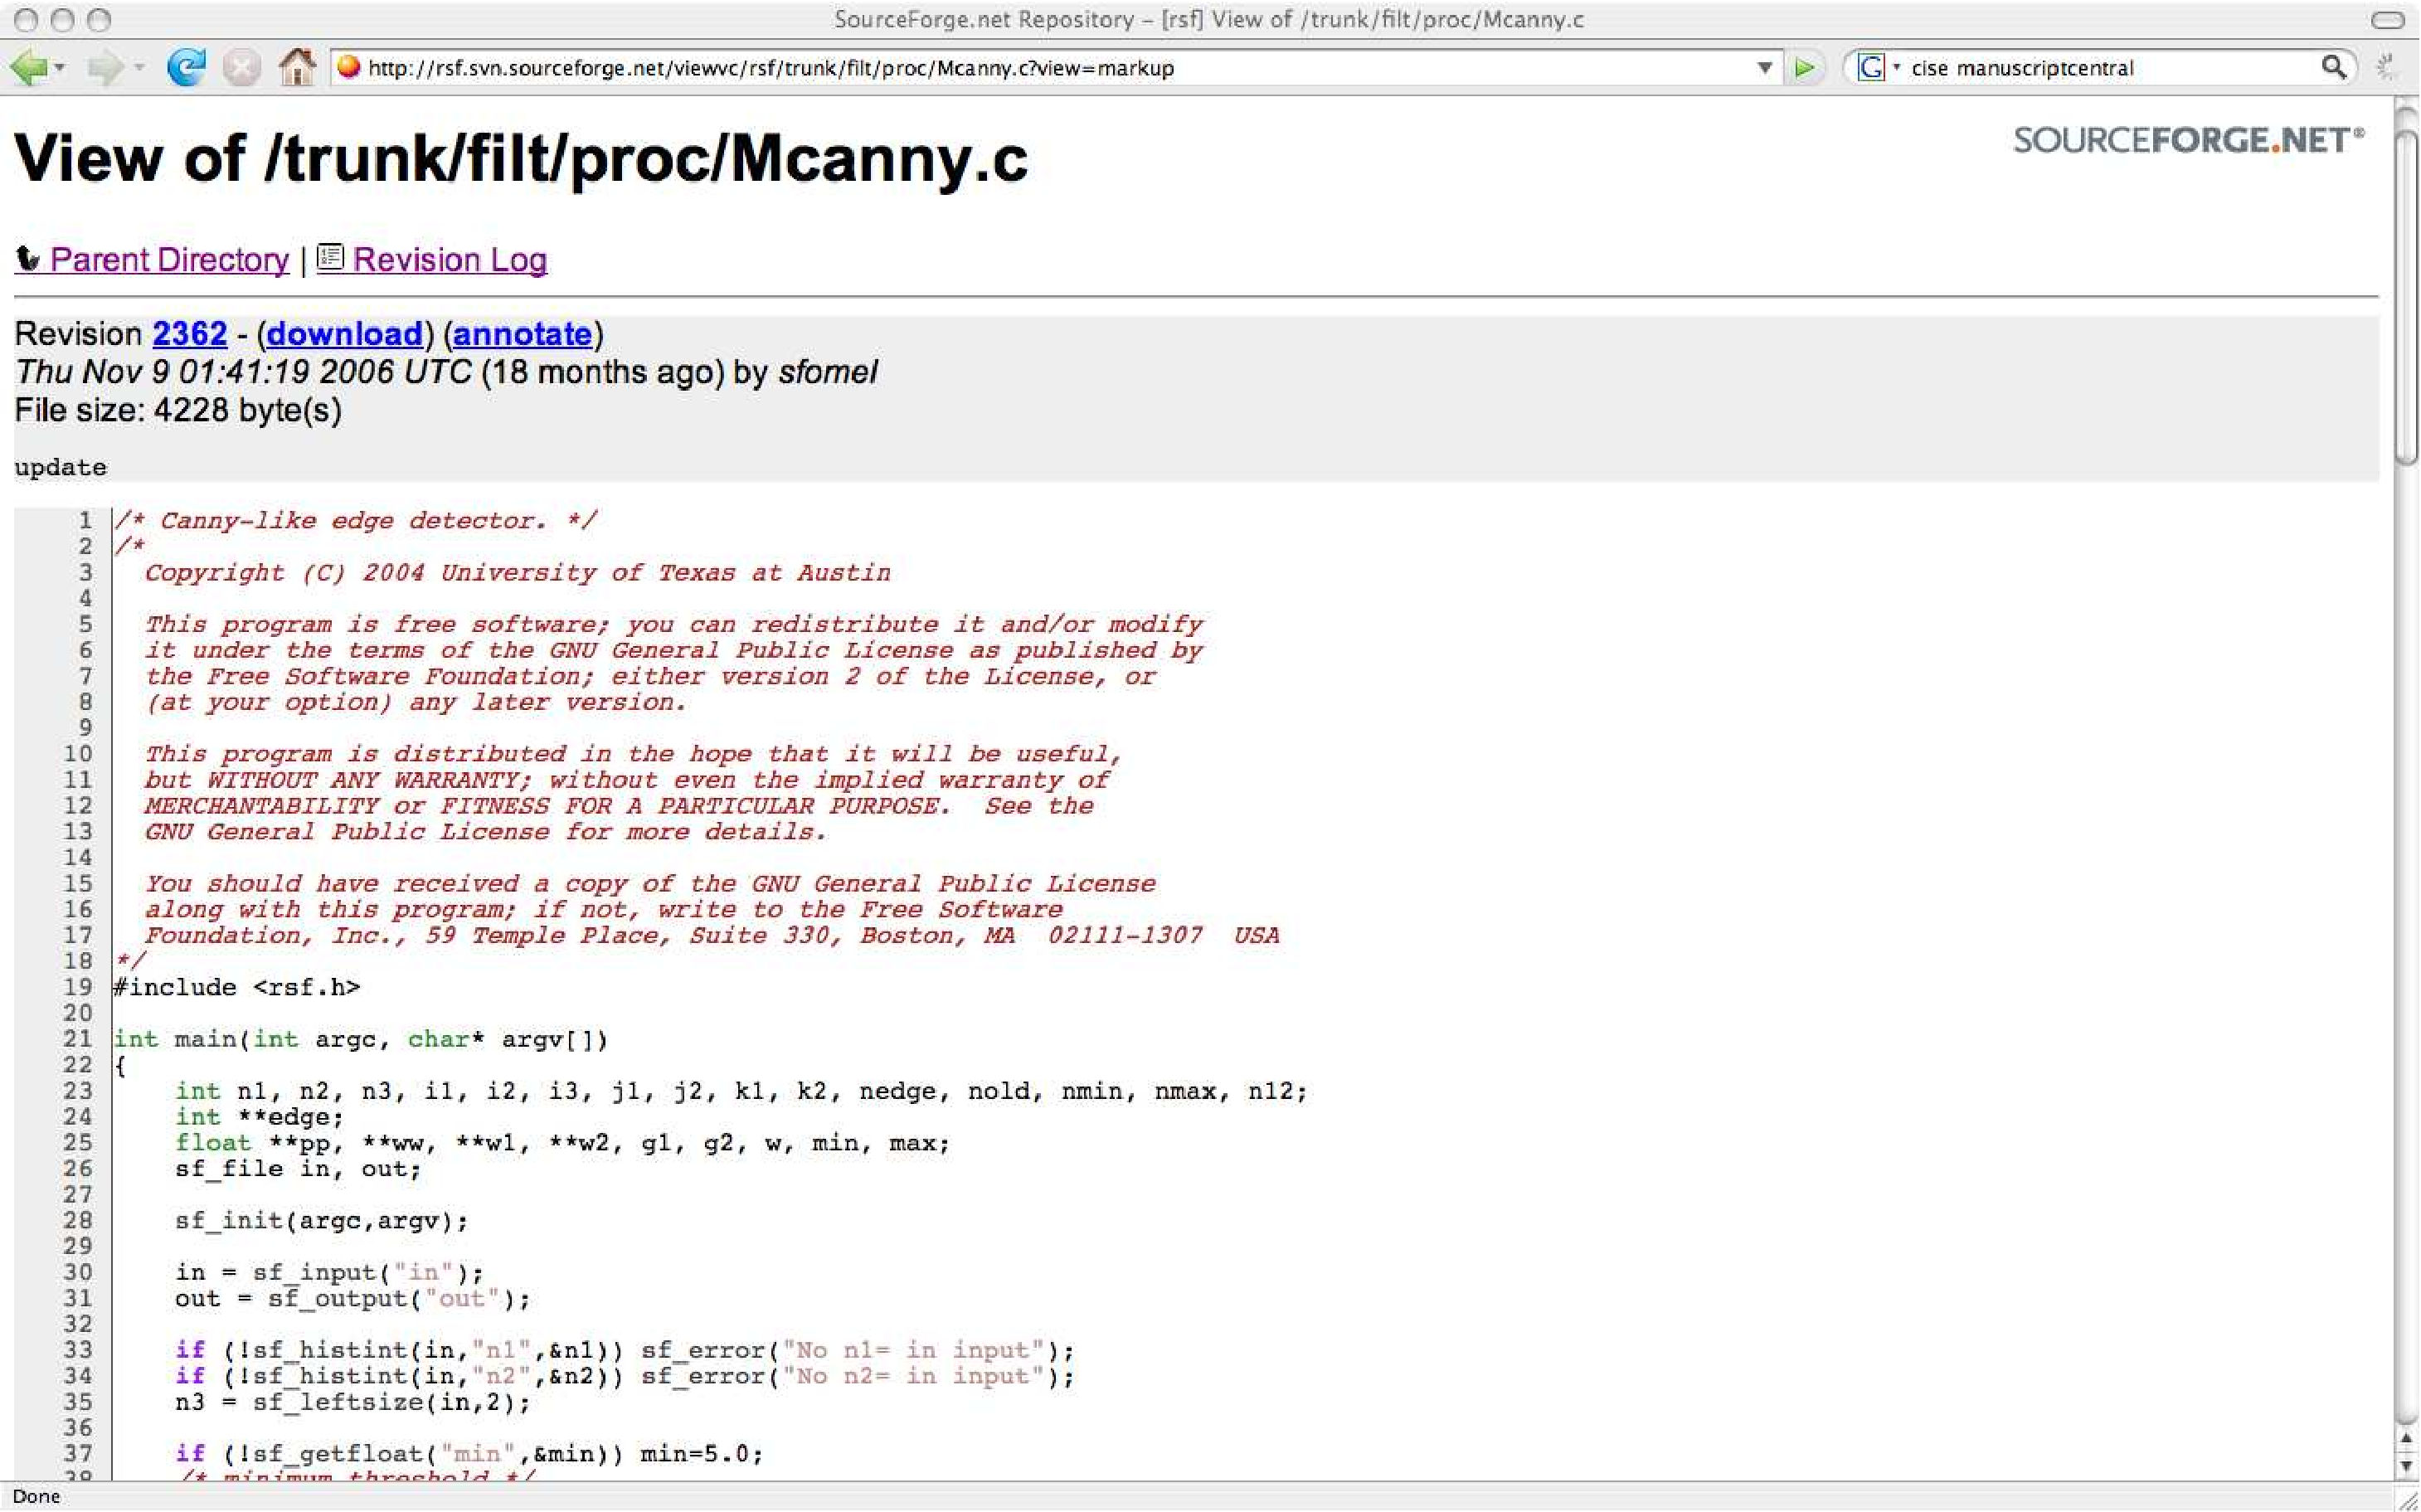
\includegraphics[height=0.9\textheight]{Fig/canny}
\end{center}
\end{frame}

\begin{frame}
  \MadLogo
  \begin{center}
 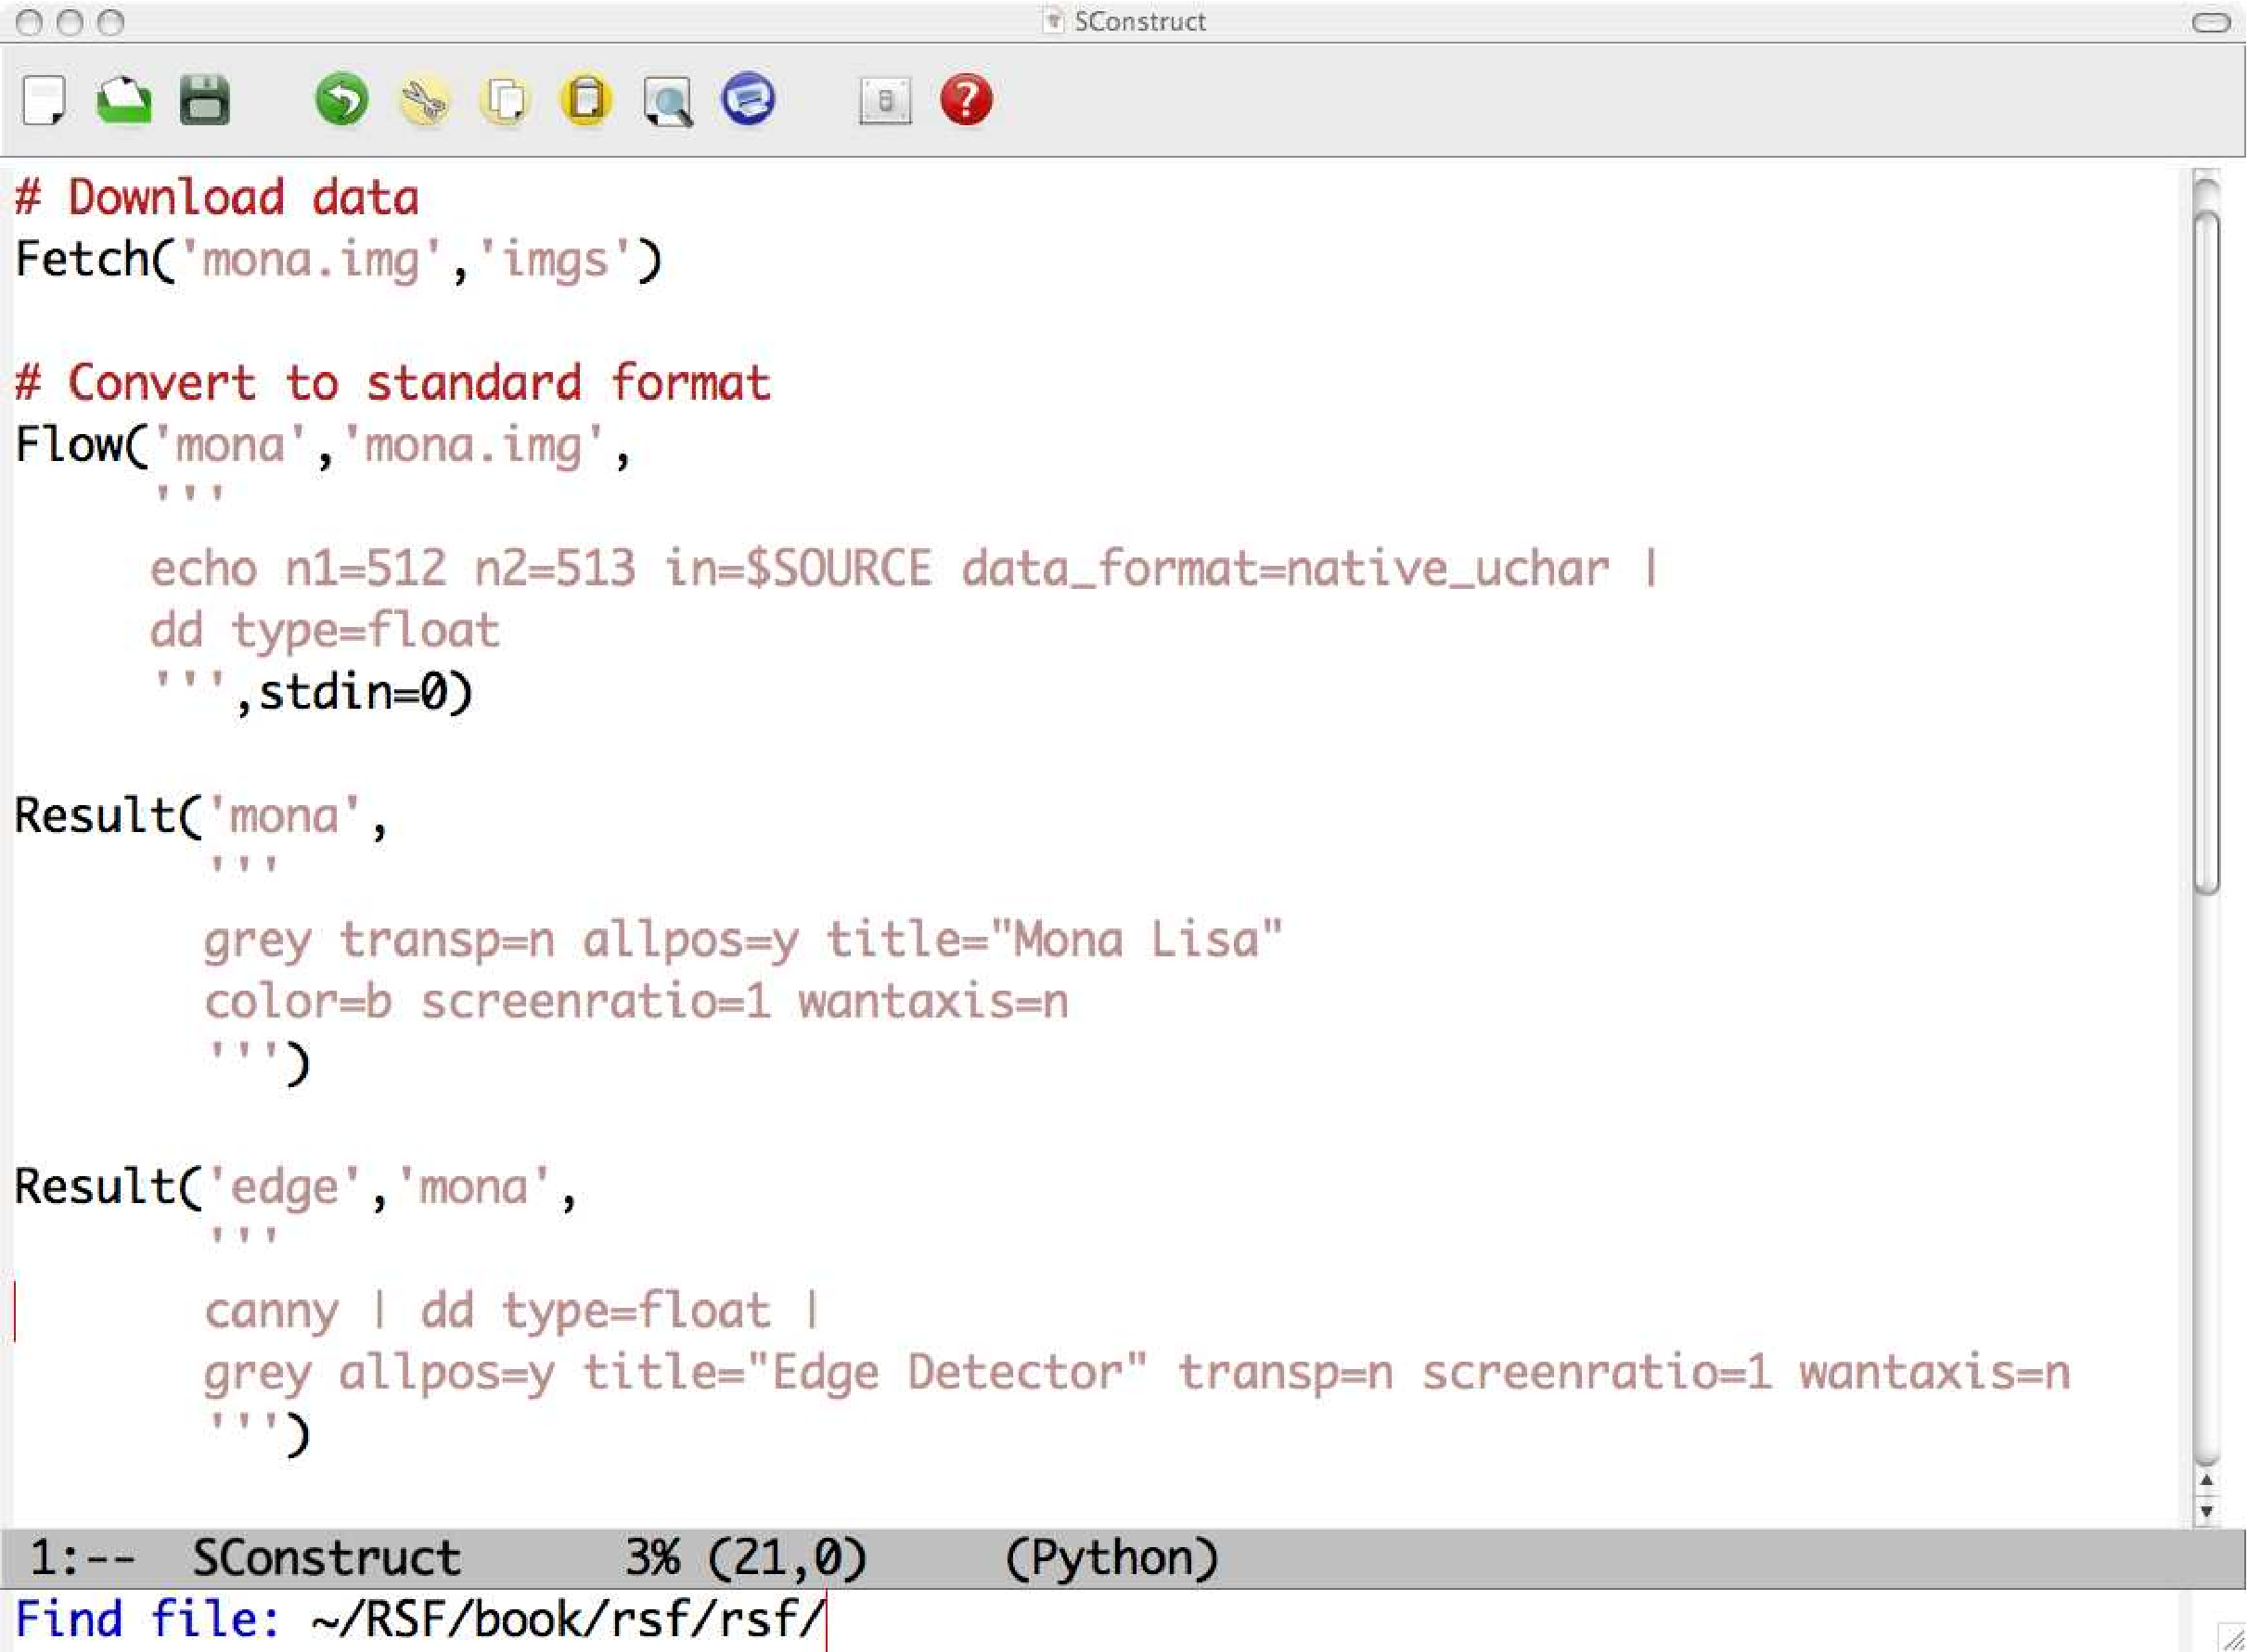
\includegraphics[height=0.9\textheight]{Fig/mona1}
  \end{center}
\end{frame}

\begin{frame}
  \MadLogo
  \begin{center}
    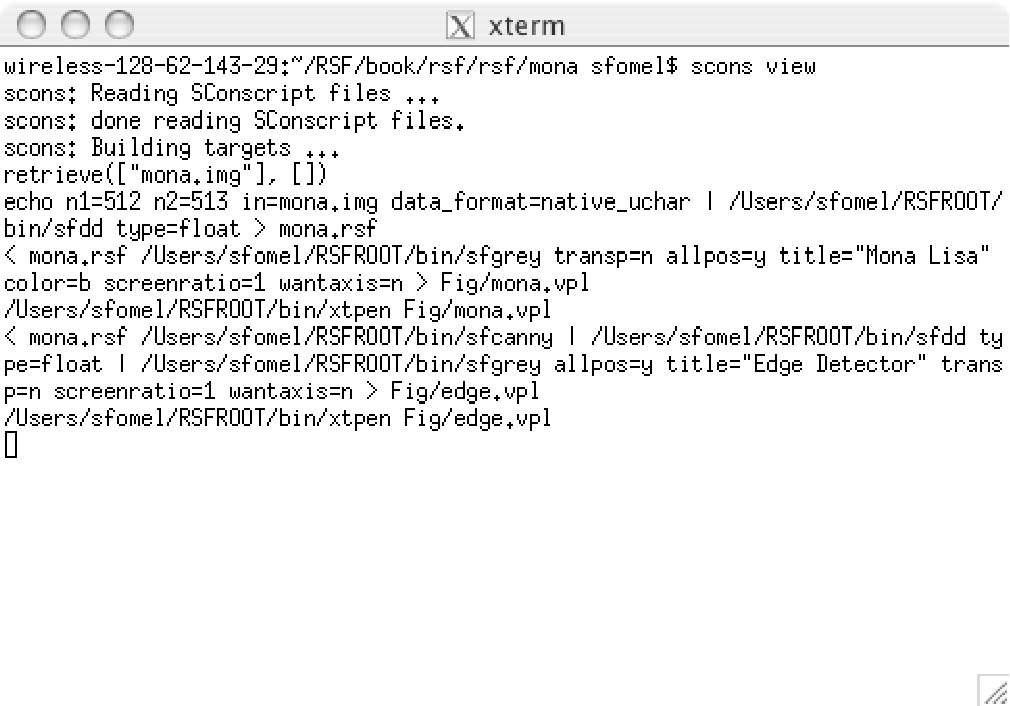
\includegraphics[width=0.8\textwidth]{Fig/scons1}
  \end{center}
\end{frame}


\begin{frame}
  \MadLogo
  \begin{center}
    \includegraphics[width=0.45\textwidth]{mona/Fig/mona}
    \hfill
    \includegraphics[width=0.45\textwidth]{mona/Fig/edge}
  \end{center}
\end{frame}

\begin{frame}
  \MadLogo
  \begin{center}
 \includegraphics[height=0.9\textheight]{Fig/mona2}
  \end{center}
\end{frame}

\begin{frame}
  \MadLogo
  \begin{center}
    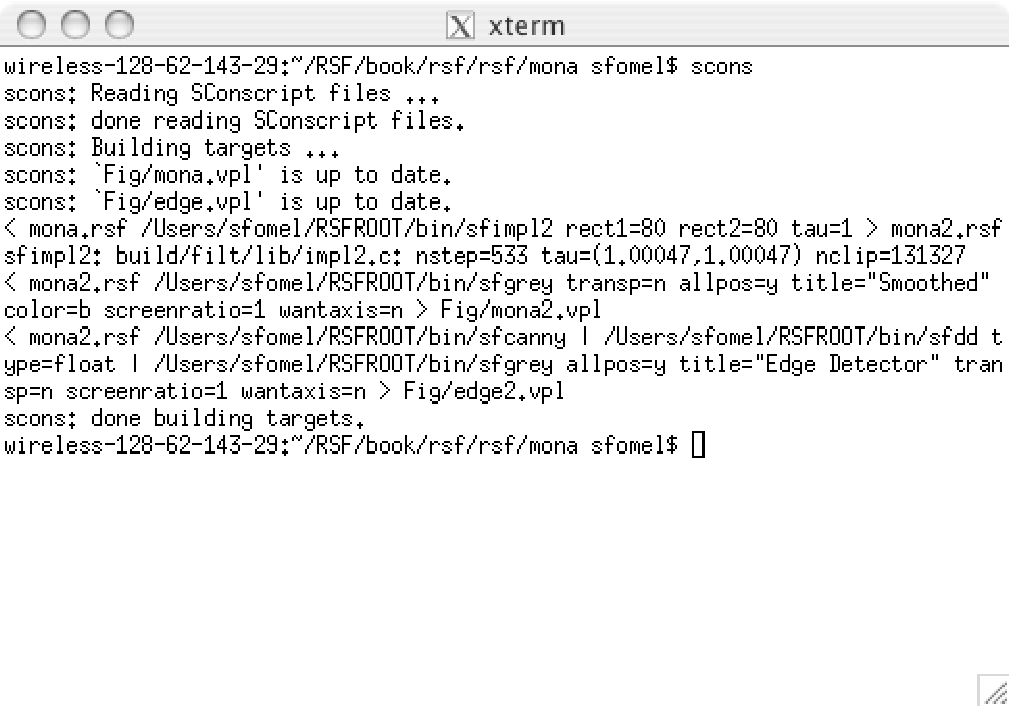
\includegraphics[width=0.8\textwidth]{Fig/scons2}
  \end{center}
\end{frame}

\begin{frame}
  \MadLogo
  \begin{center}
    \includegraphics[width=0.45\textwidth]{mona/Fig/mona2}
    \hfill
    \includegraphics[width=0.45\textwidth]{mona/Fig/edge2}
  \end{center}
\end{frame}

\begin{frame}
  \MadLogo
  \begin{center}
 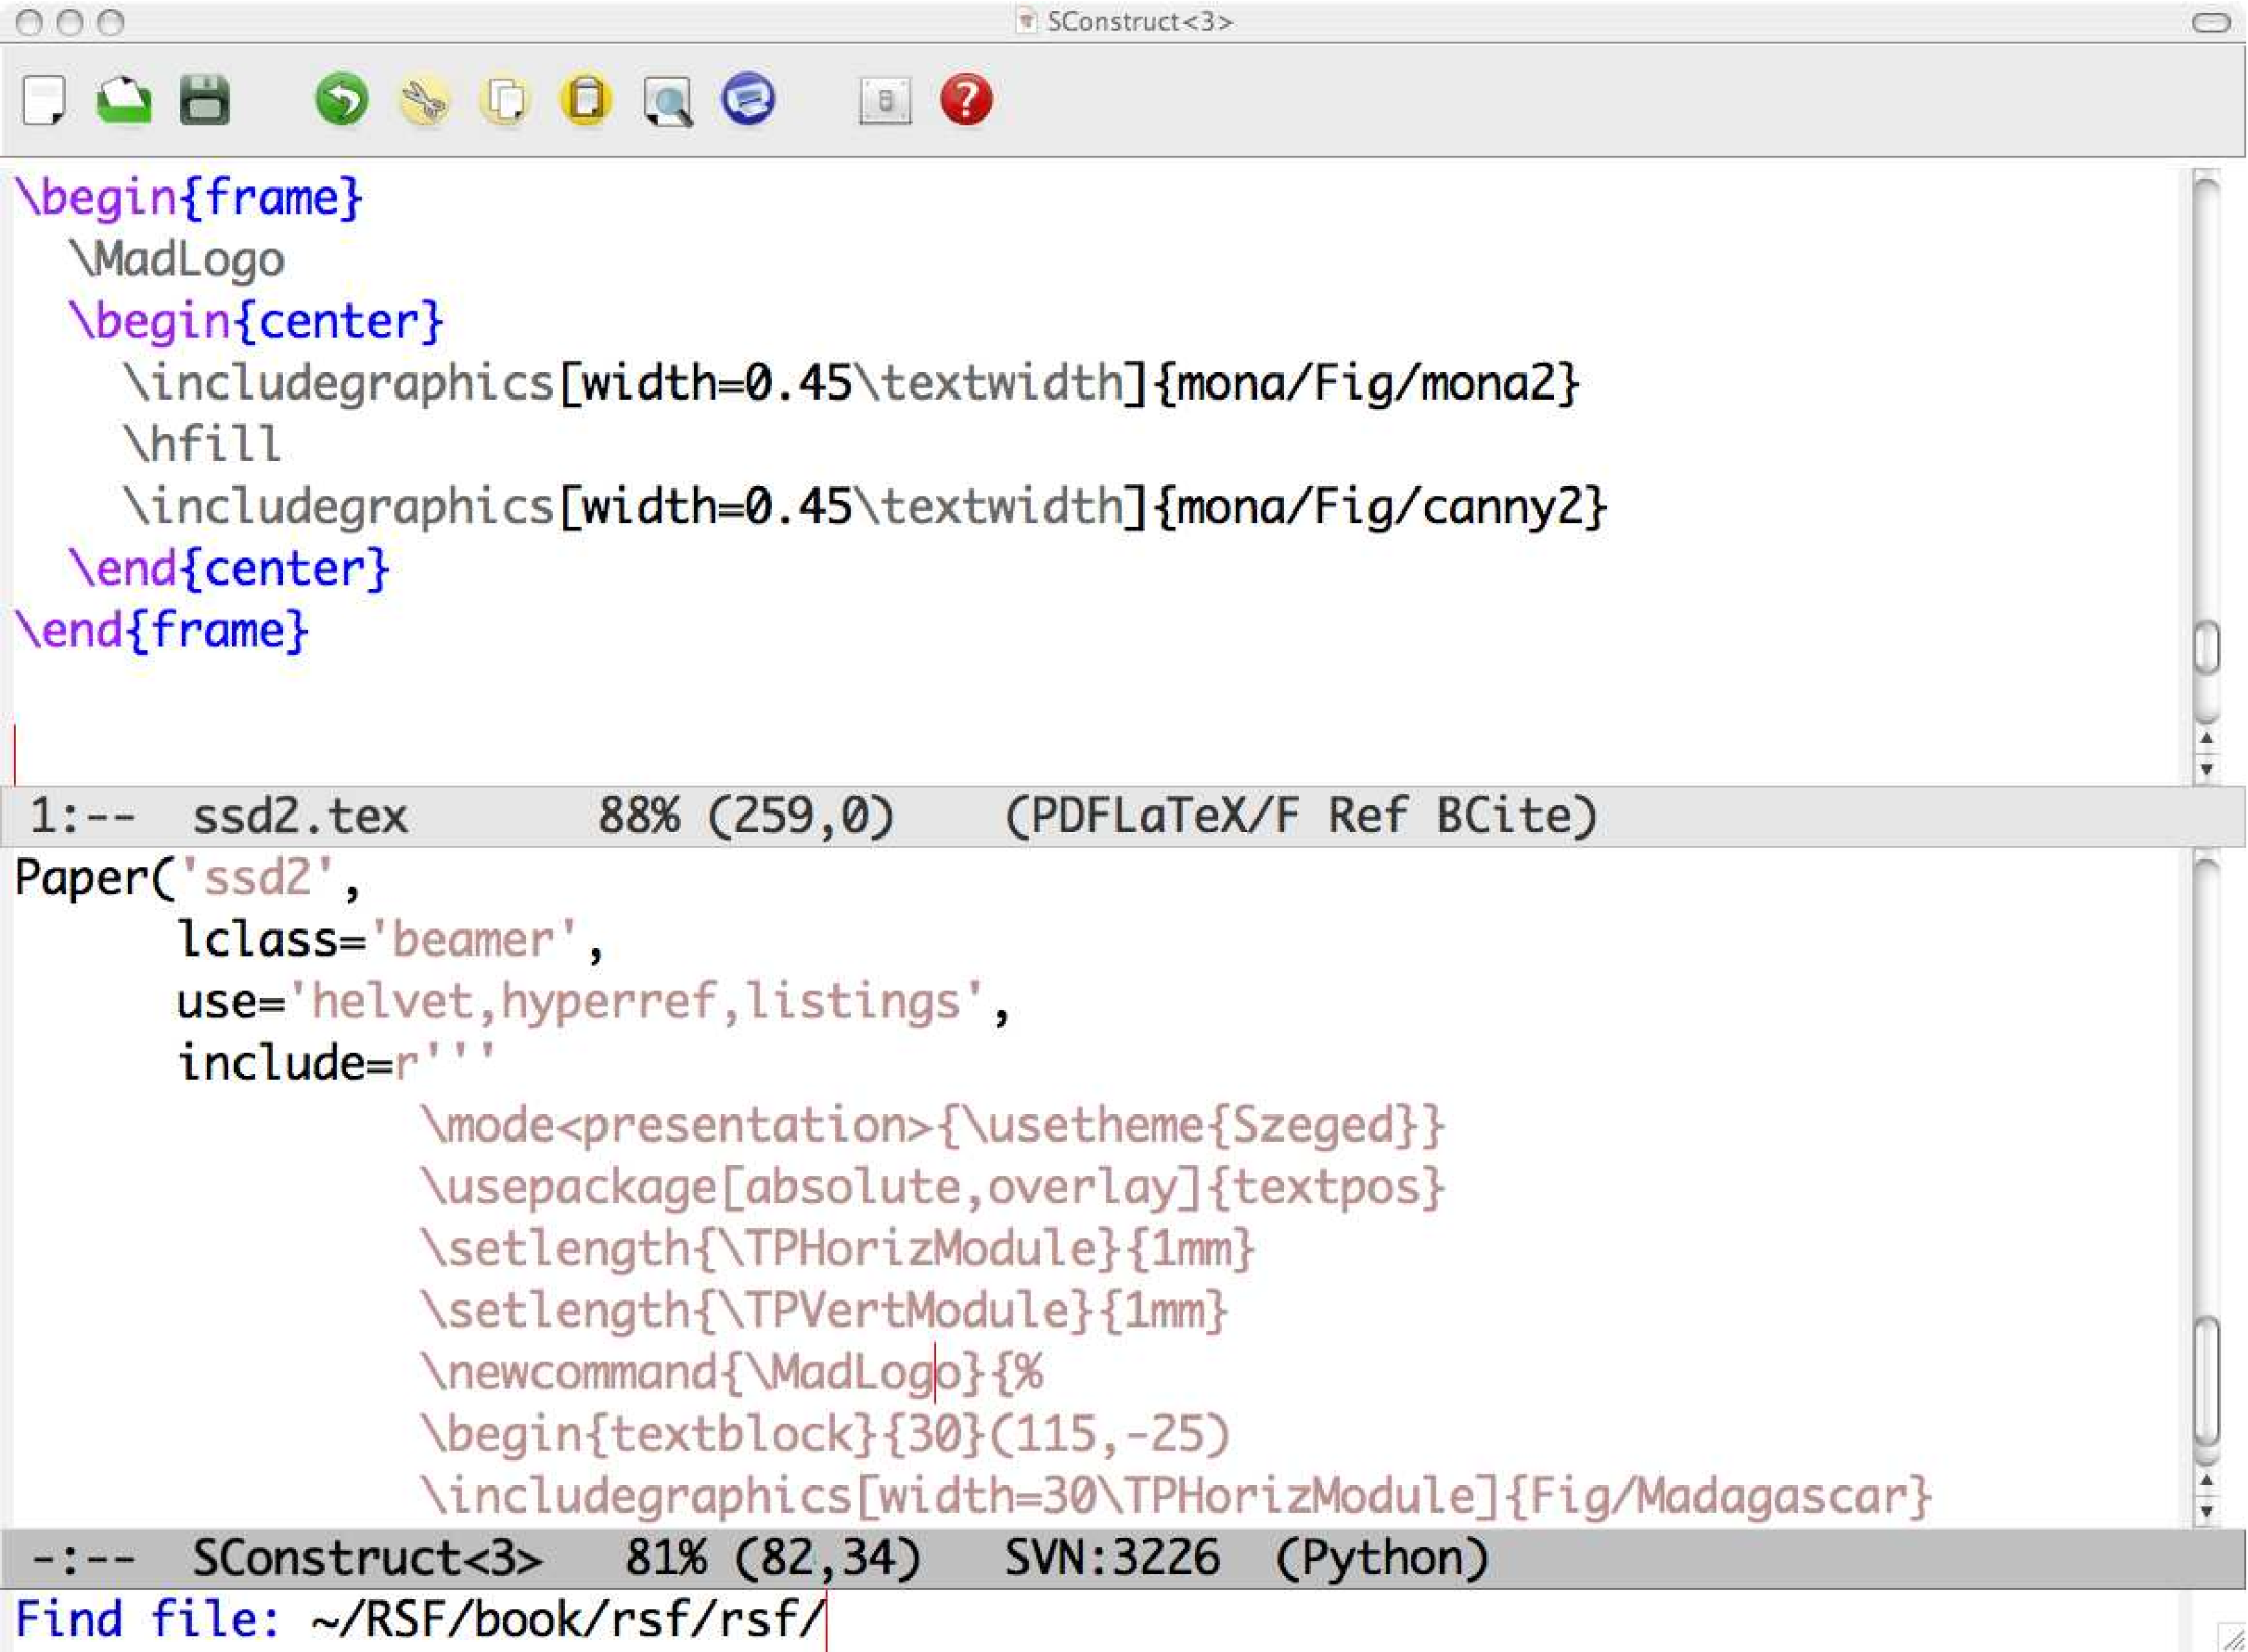
\includegraphics[height=0.9\textheight]{Fig/emacs}
  \end{center}
\end{frame}

\begin{frame}
  \MadLogo

  \frametitle{\textsc{Madagascar} Tools}

    \begin{enumerate}
    \item Number crunching
      \begin{itemize}
      \item Main programs (C, Fortran, C++, etc)
      \item \href{http://www.reproducibility.org/RSF/}{500 modules}
      \end{itemize}
    \item Visualization and experiment setup 
      \begin{itemize}
      \item Data processing flows (Python/SCons)
      \item 600 scripts, 1,700 tests
      \end{itemize}
    \item Publications and presentations
      \begin{itemize}
      \item Books and papers (\LaTeX\ and Python/SCons)
      \item \href{http://rsf.sourceforge.net/Reproducible_Documents}{100 papers}
      \end{itemize}
    \end{enumerate}

\end{frame}

\section{Conclusions}
\begin{frame}<beamer>
  \MadLogo
  \frametitle{Outline}
  \tableofcontents[currentsection]
\end{frame}

\begin{frame}
  \MadLogo
  \frametitle{Conclusions}

  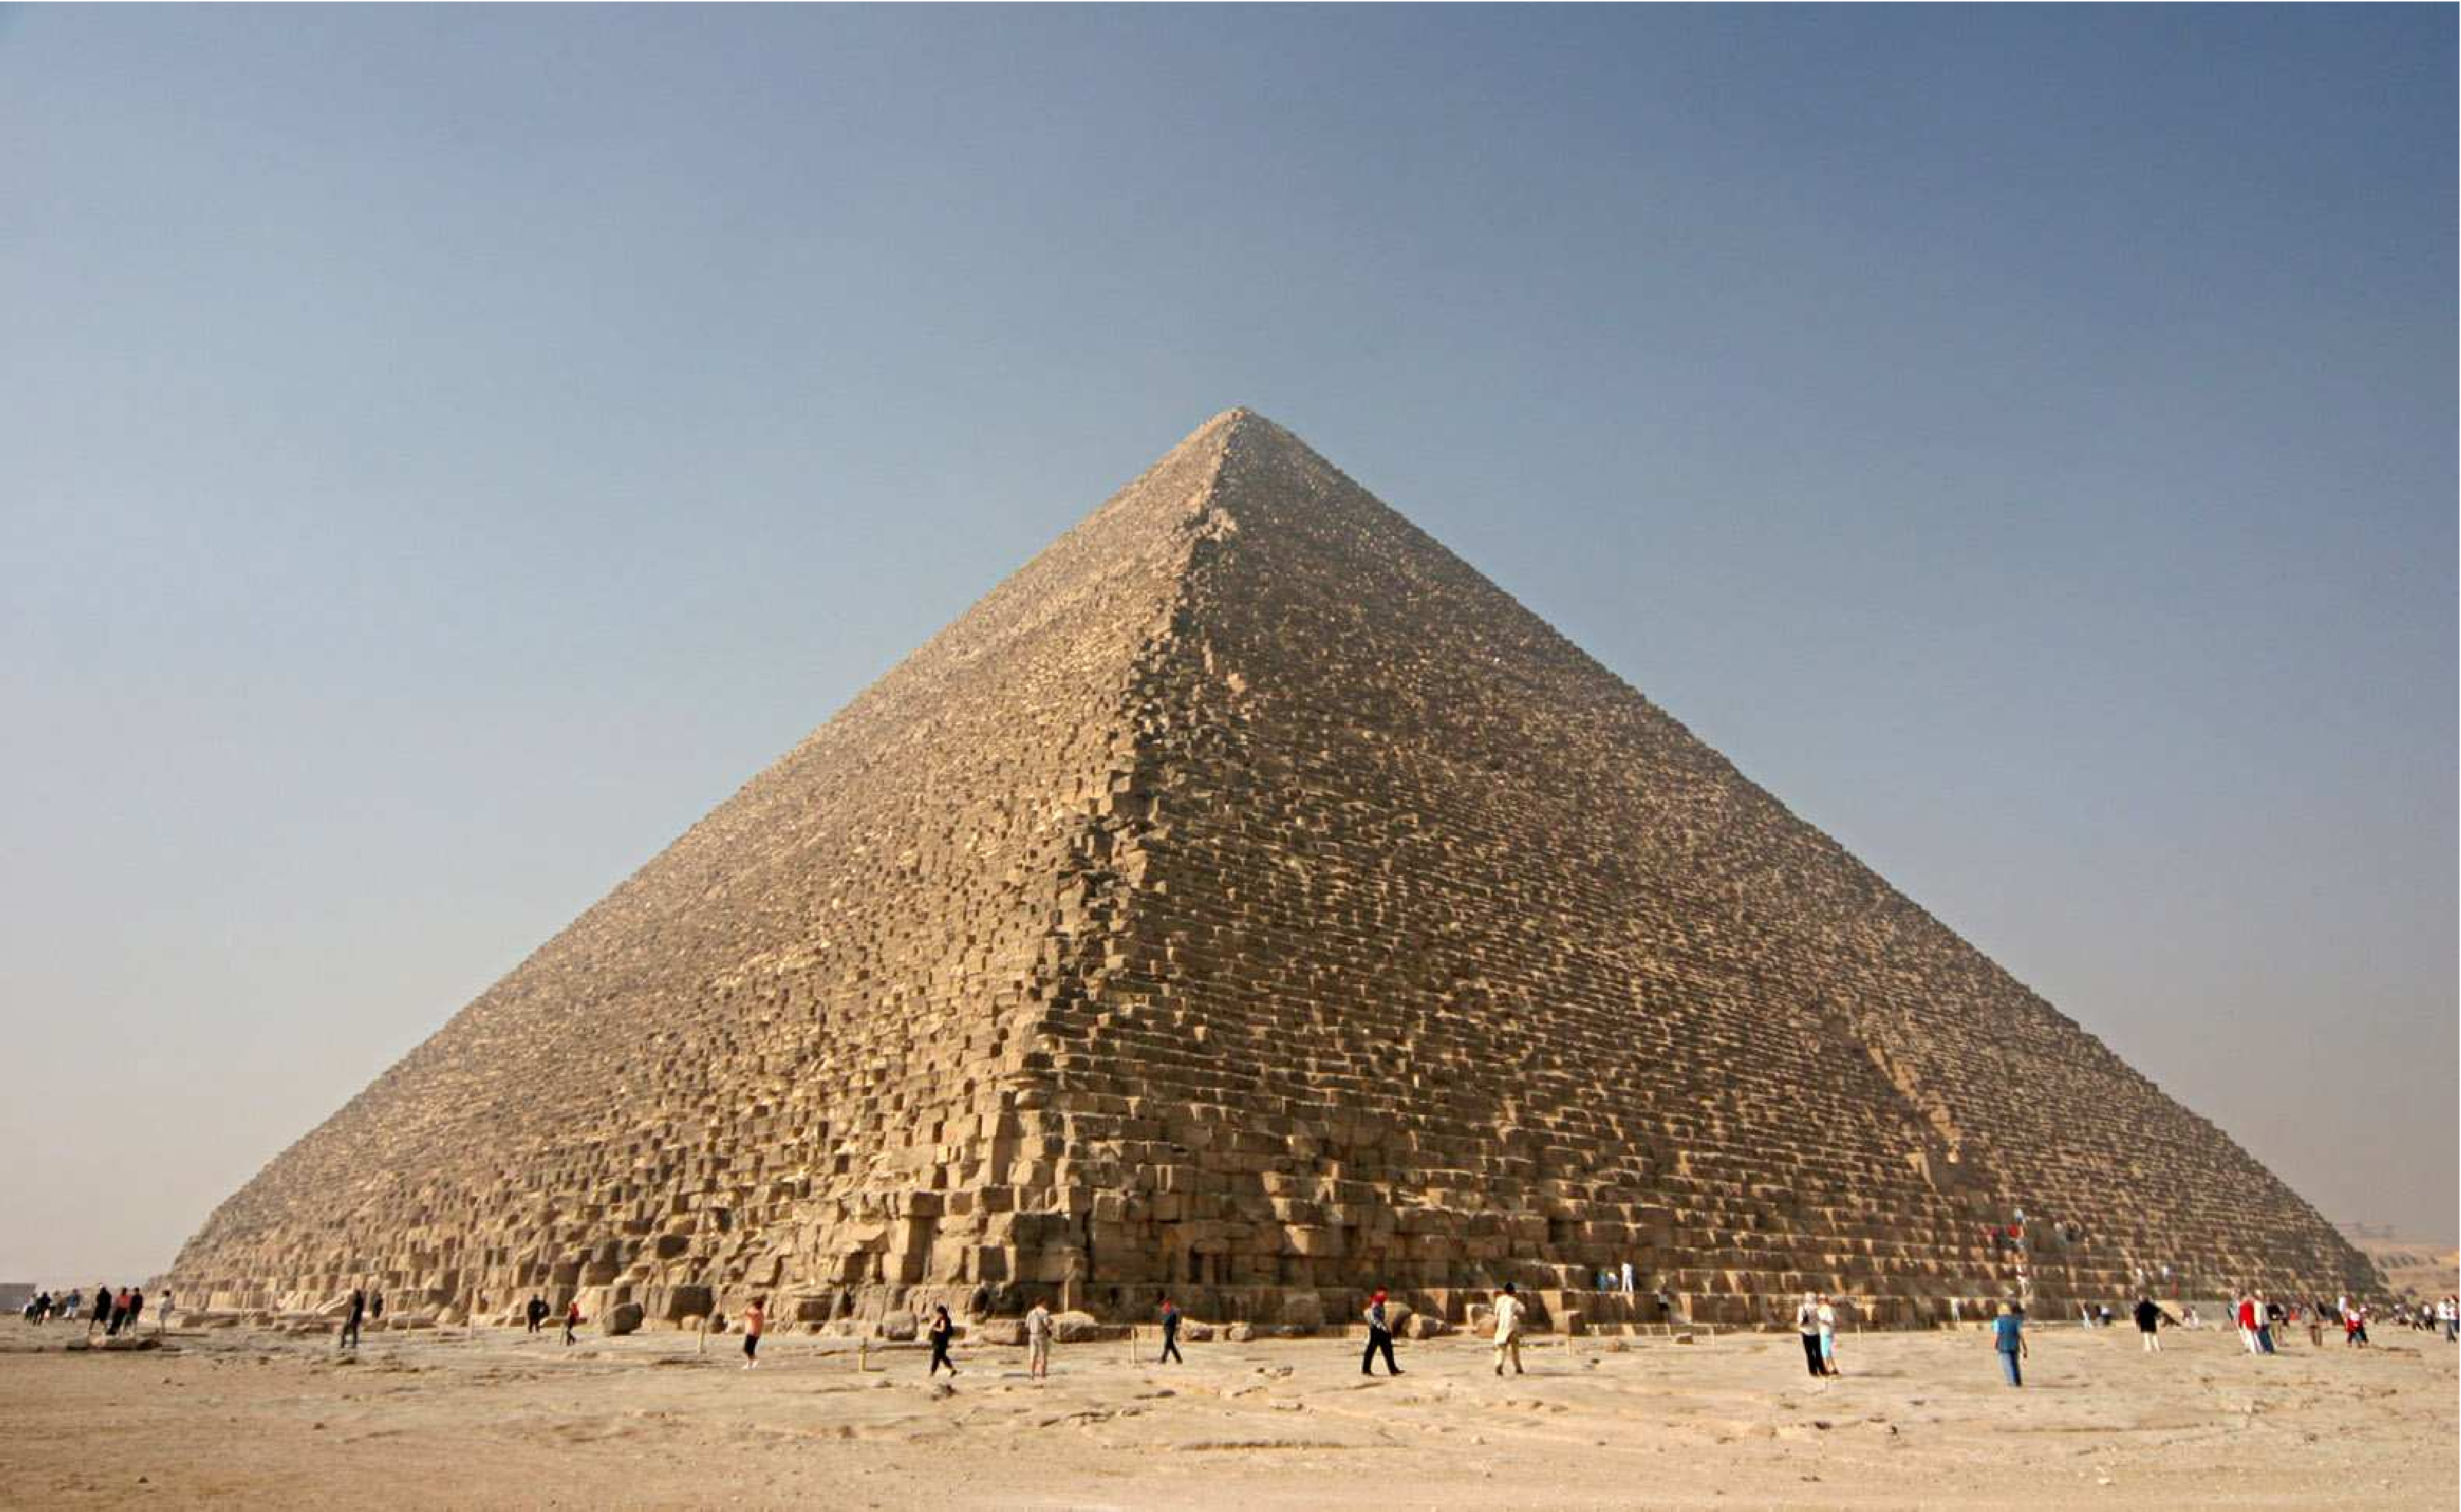
\includegraphics[height=0.6\textheight]{Fig/Kheops-Pyramid}

  \begin{itemize}
  \item Reproducible computational experiments
  \item Reproducibility = maintenance
  \item \textsc{Madagascar} software package
  \end{itemize}
\end{frame}

\begin{frame}
  \MadLogo
  \frametitle{Help Needed}
  
  \begin{itemize}
    \item Automatic testing
    \item Efficient parallelization
    \item Visualization standards
    \item Graphical User Interface
    \item \ldots
  \end{itemize}
  
\begin{center}
\color{blue}{{\Large \url{http://rsf.sourceforge.net}}}
\end{center}

\end{frame}



